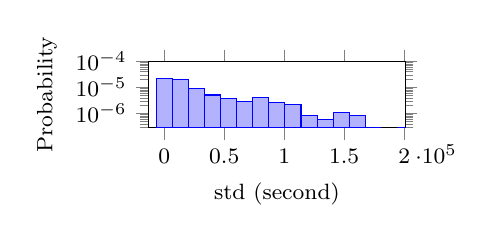
\begin{tikzpicture}
\begin{axis}[ymax=0.0001,ybar,ymode=log,bar width=13410.783587930588,log origin=infty,xmin=-13410.783587930588,ytick align=outside,enlargelimits=0,
width=.40\textwidth,
height=.20\textwidth,
ylabel=Probability,
xlabel=std (second),
every x tick scale label/.style={at={(xticklabel cs:1)},anchor=south west},
  label style={font=\footnotesize},
tick label style={font=\footnotesize} ,
]
\addplot  plot coordinates {
(0.0, 2.1630081044550223e-05)
(13410.783587930588, 1.9637836737815332e-05)
(26821.567175861175, 8.822796215540222e-06)
(40232.350763791765, 5.122913931604e-06)
(53643.13435172235, 3.699882283936222e-06)
(67053.91793965294, 2.8460632953355556e-06)
(80464.70152758353, 3.984488613469778e-06)
(93875.48511551411, 2.561456965802e-06)
(107286.2687034447, 2.2768506362684445e-06)
(120697.0522913753, 8.538189886006666e-07)
(134107.83587930587, 5.692126590671111e-07)
(147518.61946723645, 1.1384253181342222e-06)
(160929.40305516706, 8.538189886006666e-07)
(174340.18664309764, 2.8460632953355556e-07)
(187750.97023102822, 0.0)
(201161.75381895882, 2.8460632953355556e-07)
};\end{axis}
\end{tikzpicture}
